\chapter{INTRODUÇÃO}
\label{cap:introducao-marker}

A crescente complexidade dos ambientes de desenvolvimento e operações de software, impulsionada pela adoção de práticas de DevOps e pela proliferação da computação em nuvem, tem demandado abordagens inovadoras para garantir a segurança das aplicações e da infraestrutura subjacente. No ciclo de desenvolvimento tradicional (\textit{waterfall} ou modelos fortemente segmentados), a segurança era tratada como uma etapa isolada, executada geralmente ao final do processo por equipes especializadas. Esse modelo resultava em atrasos na entrega, em custos de correção elevados e em vulnerabilidades detectadas tardiamente, muitas vezes já em produção~\citeonline{humble2010continuous, kim2021devops}.

De acordo com o OWASP Top 10, entre as principais vulnerabilidades do mercado até o ano de 2025 estão a Quebra de Controle de Acesso, o Design Inseguro e a Configuração Insegura (\textit{Security Misconfiguration}), evidenciando a necessidade de procedimentos, padrões e ferramentas para o estabelecimento de modelos de desenvolvimento ágil e seguro~\citeonline{OWASP2025}. Configurações inseguras de infraestrutura em nuvem, em particular, apresentam-se como uma das principais causas de exposição não intencional de dados observadas nos últimos anos~\citeonline{rahman2019sharpshooter}.

Segundo o relatório \textit{IBM Cost of a Data Breach} 2024, o custo médio global das violações atingiu 4,88 milhões de dólares, um aumento significativo em relação aos 4,45 milhões de dólares de 2023 e o maior salto desde a pandemia~\citeonline{ibmDataBreachCost}. Para as empresas do setor financeiro, os custos são ainda mais elevados: 6,08 milhões de dólares em média por incidente, o que representa um aumento de 22\% em relação à média global~\citeonline{ibmDataBreachCost}.

Nesse contexto, o conceito de DevSecOps emerge como uma evolução do DevOps, integrando práticas de segurança em todas as fases do SDLC (\textit{Software Development Life Cycle}), desde o planejamento e o design até a implantação e a operação~\citeonline{kim2021devops, myrbakken2017devsecops}. Simultaneamente, a Infraestrutura como Código (IaC) tem se consolidado como uma prática fundamental para provisionar e gerenciar infraestrutura de forma automatizada e declarativa, utilizando arquivos de configuração versionados~\citeonline{morris2020infrastructure, vehent2018securing}. Estudos sistemáticos indicam que essa combinação -- IaC + segurança automatizada -- é hoje um dos temas mais promissores na engenharia de software de operações~\citeonline{rahman2019survey, sanchez2020devsecops}.

A sinergia entre DevSecOps e IaC apresenta um potencial significativo para automatizar a integração da segurança na infraestrutura desde sua concepção~\citeonline{morris2020infrastructure, artac2017devops}. Ao definir a infraestrutura de forma programática, é possível incorporar controles de segurança diretamente nas configurações, garantindo a conformidade e reduzindo a superfície de ataque. A automação propiciada pelo DevSecOps pode então aplicar esses controles de forma consistente e eficiente ao longo do ciclo de vida da infraestrutura, materializando o princípio de \textit{Shift-Left}, no qual as verificações são deslocadas para o início do fluxo de desenvolvimento~\citeonline{jimenez2019state}.

\section{Contextualização}
\label{sec:contextualizacao}

Este trabalho investiga a integração de DevSecOps e IaC por meio de uma abordagem prática, apoiada em um estudo de caso conduzido pelo próprio autor em ambiente controlado. Para viabilizar a análise em duas perspectivas complementares -- uma orientada à realidade corporativa e outra à reprodutibilidade acadêmica -- foram desenvolvidas \textbf{duas Provas de Conceito (PoC)} independentes, porém alinhadas conceitualmente:

\begin{itemize}
    \item \textbf{PoC em nuvem AWS} \citeonline{PocDevSecOpsAWS2026}: representa um ambiente corporativo real, com serviços gerenciados (VPC, EKS, RDS, S3, IAM, KMS, CloudTrail, GuardDuty, Security Hub) provisionados via Terraform. É a materialização do modelo proposto em um cenário produtivo, com múltiplos ambientes (\texttt{dev}/\texttt{prod}), federação de identidade via OpenID Connect (OIDC) e a esteira DevSecOps completa em GitHub Actions.

    \item \textbf{PoC baseada em contêineres} \citeonline{PocDevSecOps2026}: espelha a mesma arquitetura AWS em ambiente local, substituindo cada serviço da nuvem por um contêiner Docker equivalente (por exemplo, \texttt{docker\_network} no lugar da VPC, PostgreSQL em contêiner no lugar do RDS e \texttt{nginx} no lugar do ALB). O objetivo desta segunda PoC é permitir que qualquer pessoa reproduza a experiência integralmente em sua máquina, sem depender de cadastro, custos ou permissões em provedores de nuvem pública, o que a torna particularmente adequada ao contexto acadêmico e ao ensino de DevSecOps.
\end{itemize}

Ambas as PoC compartilham as mesmas ferramentas de análise (Checkov, GitGuardian/Gitleaks, OPA/Conftest, Trivy, Hadolint) e os mesmos critérios de qualidade, o que permite comparar o comportamento dos controles nos dois cenários e discutir as implicações práticas da abordagem \textit{Shift-Left}.

\section{Perguntas da Pesquisa}

As perguntas desta pesquisa visam explorar os problemas enfrentados atualmente por empresas e instituições e elaborar alternativas para contornar ou mitigar essas fraquezas por meio da automação da segurança em pipelines de IaC.

A Figura~\ref{fig:owasp} apresenta as principais vulnerabilidades do mercado até o ano de 2025 de acordo com o OWASP Top 10. É possível observar que, entre as principais, estão: Quebra de Controle de Acesso, Design Inseguro e Configuração Insegura.

\begin{figure}[ht]
    \caption{Riscos críticos de segurança em aplicações web, conforme o OWASP Top 10 de 2025, apresentando as vulnerabilidades em categorias prioritárias e facilitando a compreensão e mitigação de ameaças por desenvolvedores e equipes de segurança.}
    \label{fig:owasp}
    \centering
    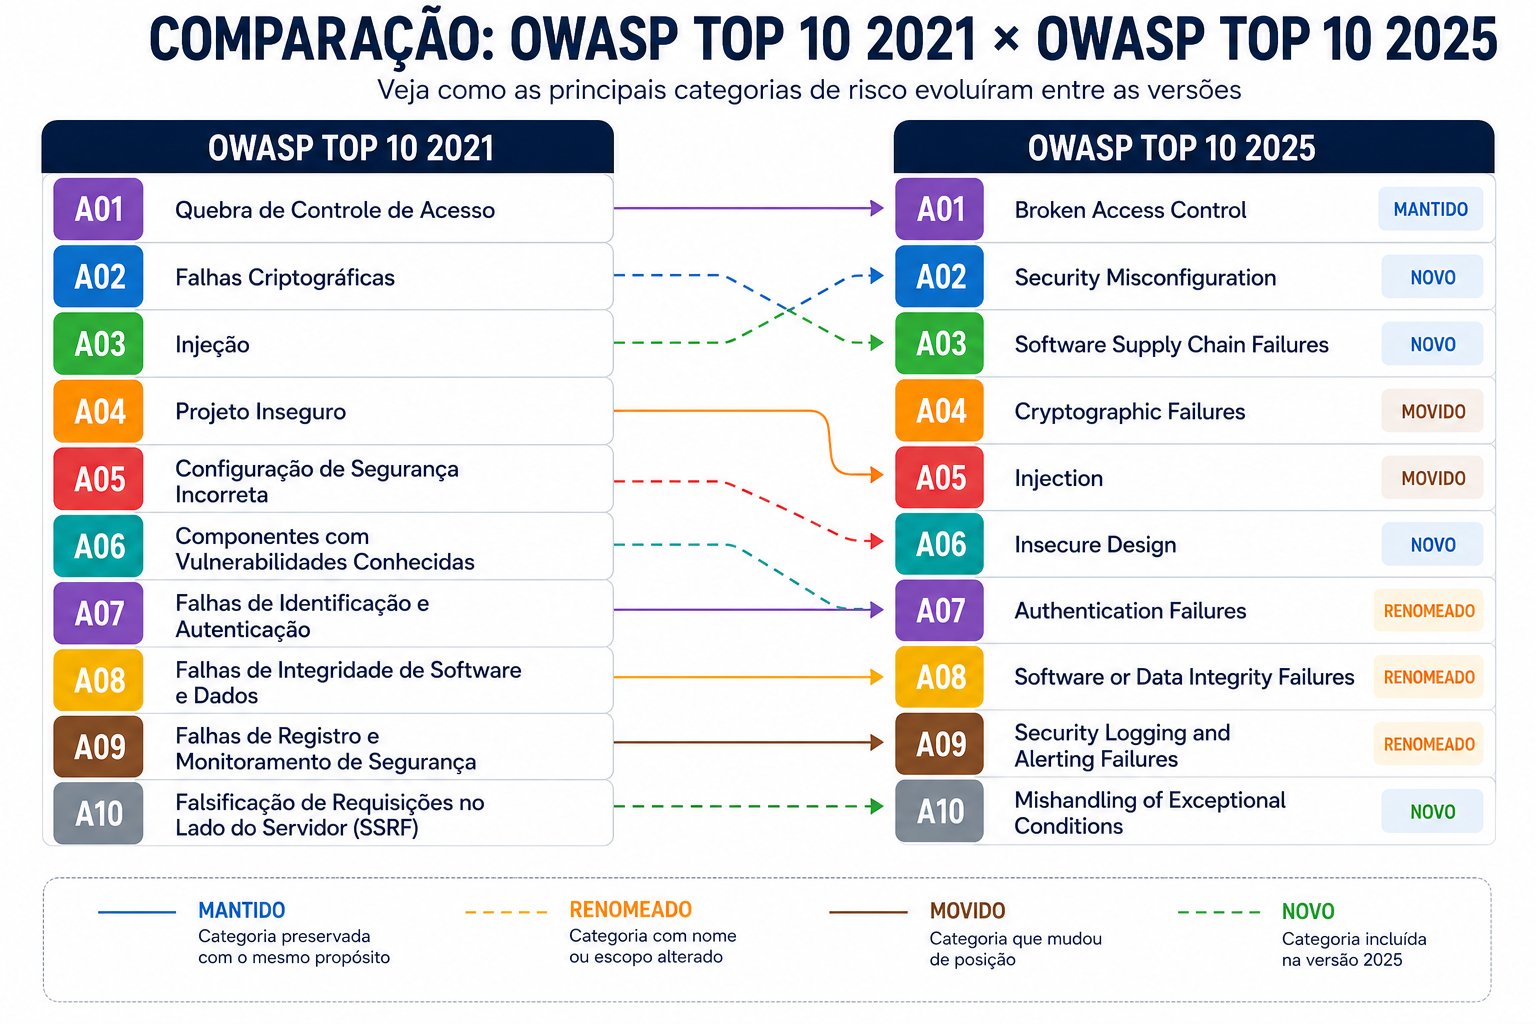
\includegraphics[width=0.8\textwidth]{Arquivos/figuras/Figura_OWASP_Top_10_2025_Diagram.png}
    \fonte{\citeonline{OWASP2025}}
\end{figure}

O OWASP Top 10 é uma lista mantida pela \textit{Open Web Application Security Project} que identifica as dez principais vulnerabilidades de segurança em aplicações web, com base em dados coletados globalmente da comunidade de segurança e de scanners automatizados~\citeonline{OWASP2025}. Atualizado periodicamente, o OWASP Top 10 serve como um guia prático para desenvolvedores, arquitetos e equipes de segurança compreenderem, priorizarem e mitigarem os riscos mais críticos. Entre as categorias, incluem-se falhas como controle inadequado de acesso, injeção de código (por exemplo, \textit{SQL Injection}), exposição de dados sensíveis e falhas na autenticação. Cada item da lista inclui exemplos, impacto potencial e orientações sobre como prevenir ou remediar essas vulnerabilidades, auxiliando organizações no fortalecimento de suas aplicações e na redução de sua superfície de ataque.

Neste contexto, as perguntas que orientam a pesquisa são:

\begin{itemize}
    \item Como integrar de forma eficaz e automatizada práticas de segurança (DevSecOps) na definição e na gestão da infraestrutura por meio de Infraestrutura como Código (IaC), a fim de garantir a segurança e a conformidade desde as fases iniciais do ciclo de vida da infraestrutura?
    \item Quais são as principais barreiras e desafios para a adoção de práticas DevSecOps no contexto de IaC e como superá-los?
    \item De que forma a integração de ferramentas e processos de DevSecOps com IaC pode melhorar a rastreabilidade, a auditabilidade e a conformidade em ambientes de infraestrutura complexos?
    \item Quais métricas e indicadores podem ser utilizados para avaliar a eficácia da integração entre DevSecOps e IaC em termos de segurança e desempenho?
    \item Como práticas de DevSecOps baseadas em IaC podem ser escaladas para diferentes níveis de maturidade organizacional e complexidade tecnológica?
    \item Em que medida o modelo proposto para um ambiente de nuvem pública (AWS) é transponível para um cenário local (contêineres), sem descaracterizar os controles e as garantias de segurança?
\end{itemize}

\section{Justificativa}

A crescente complexidade dos sistemas computacionais exige abordagens inovadoras para gerenciar segurança, eficiência e escalabilidade. Esta pesquisa se justifica pela necessidade de reduzir vulnerabilidades e o tempo de resposta a incidentes, ao mesmo tempo em que promove práticas de automação. A integração de DevSecOps e IaC tem potencial para atender a essas demandas de forma sustentável e eficaz por meio de pipelines automatizados de DevSecOps\footnote{\textbf{Pipeline de DevSecOps:} fluxo automatizado que incorpora segurança em todas as etapas do desenvolvimento e entrega de software, unindo práticas de DevOps a controles de segurança contínuos~\citeonline{myrbakken2017devsecops}.}.

A integração de DevSecOps e IaC representa uma abordagem promissora para enfrentar os desafios de segurança em ambientes de TI modernos e dinâmicos. A automação da segurança na infraestrutura, desde sua concepção por meio da IaC, pode levar a diversos benefícios, entre eles:

\begin{itemize}
    \item \textbf{Redução de vulnerabilidades:} a incorporação de controles de segurança desde o início do ciclo de vida diminui a probabilidade de configurações inseguras serem implementadas em produção~\citeonline{rahman2019sharpshooter}.
    \item \textbf{Aumento da conformidade:} a automação da aplicação de políticas garante a aderência a padrões de segurança e a regulamentações como o CIS Benchmarks~\citeonline{CIS2024AWS} e a LGPD~\citeonline{lgpd2018}.
    \item \textbf{Melhora na eficiência:} a automação de tarefas de segurança libera equipes para se concentrarem em outras atividades de maior valor agregado~\citeonline{forsgren2018accelerate}.
    \item \textbf{Redução de custos:} a detecção e a correção precoce de problemas de segurança são geralmente mais baratas do que lidar com incidentes em ambientes de produção~\citeonline{ibmDataBreachCost}.
    \item \textbf{Aceleração da entrega:} a integração da segurança no processo de desenvolvimento e implantação da infraestrutura evita atrasos causados por verificações tardias~\citeonline{jimenez2019state}.
\end{itemize}

A Figura~\ref{fig:cvss-intro} descreve a distribuição de severidade de vulnerabilidades ao longo do tempo, baseada no sistema CVSS, e está diretamente relacionada às perguntas da pesquisa, pois fornece a base visual e quantitativa para investigar a evolução e o impacto das classificações de risco.

O \textit{Common Vulnerability Scoring System} (CVSS) é um sistema de pontuação padronizado que permite classificar a severidade de vulnerabilidades em software e hardware, fornecendo uma medida objetiva do risco associado. O gráfico apresenta a distribuição da severidade dos riscos ao longo dos anos em três níveis, cada um representado por uma cor: Baixo (azul), Médio (amarelo) e Alto (verde).

\begin{figure}[ht]
    \caption{Distribuição de severidade das vulnerabilidades ao longo do tempo, baseada no sistema CVSS (\textit{Common Vulnerability Scoring System}), permitindo a análise visual do impacto e da evolução das classificações de risco em diferentes períodos.}
    \label{fig:cvss-intro}
    \centering
    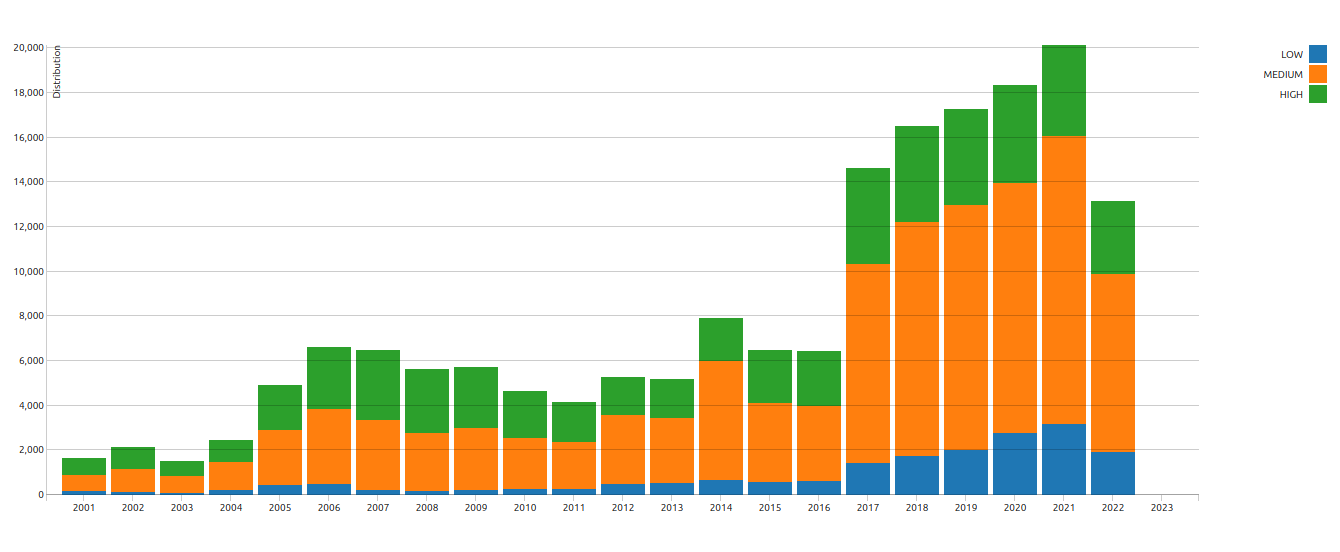
\includegraphics[width=0.8\textwidth]{Arquivos/figuras/Figura_CVSS_Severity_Distribution_Over_Time.png}
    \fonte{\citeonline{NIST2025}}
\end{figure}

A proposição de um modelo de integração claro e prático, e sua validação em dois cenários complementares (nuvem pública AWS e ambiente local em contêineres), pode fornecer um guia valioso para organizações que buscam adotar uma abordagem mais proativa e automatizada para a segurança da sua infraestrutura.

\section{Objetivos}

\subsection{Objetivo Geral}

Propor e validar, por meio de um estudo de caso técnico com duas Provas de Conceito, um modelo de integração entre DevSecOps e IaC capaz de automatizar e fortalecer práticas de segurança em infraestruturas computacionais. O modelo busca sustentar a automação da segurança e da conformidade ao longo de todo o ciclo de vida da infraestrutura, apoiando-se em práticas como \textit{Shift-Left}\footnote{\textbf{Shift-Left:} estratégia utilizada em DevSecOps que antecipa práticas de segurança no ciclo de desenvolvimento, identificando e corrigindo vulnerabilidades desde as etapas iniciais do desenvolvimento de software, reduzindo riscos e custos~\citeonline{jimenez2019state}.}, Policy-as-Code\footnote{\textbf{Policy-as-Code:} escrita de políticas de segurança e governança em linguagem declarativa (por exemplo, \textit{Rego}), permitindo que sejam versionadas, revisadas e aplicadas automaticamente na pipeline~\citeonline{OPA2024}.} e \textit{Fail-Fast}\footnote{\textbf{Fail-Fast:} princípio em que o pipeline é interrompido imediatamente ao detectar uma falha crítica, evitando a propagação do problema para etapas posteriores.}.

\subsection{Objetivos Específicos}

Considerando o desenvolvimento da pesquisa e o objetivo geral apresentado, destacam-se os seguintes objetivos específicos:

\begin{itemize}
    \item Identificar as principais práticas, ferramentas e desafios envolvidos na integração de DevSecOps e IaC;
    \item Investigar técnicas e métodos para automatizar a aplicação de políticas de segurança e conformidade em ambientes de IaC (Policy-as-Code);
    \item Propor um modelo de integração que descreva os processos, as responsabilidades e as ferramentas envolvidas na adoção de DevSecOps em IaC;
    \item Materializar o modelo em duas PoC (uma em AWS e outra em contêineres) e submetê-lo a testes controlados com configurações deliberadamente inseguras, mensurando a capacidade de detecção precoce da esteira;
    \item Discutir as implicações do modelo em termos de agilidade, governança, custos e reprodutibilidade acadêmica.
\end{itemize}

\section{Organização do Trabalho}

Esta monografia está estruturada em cinco capítulos. O presente capítulo apresenta a contextualização, a justificativa, as perguntas e os objetivos da pesquisa. O Capítulo~2 traz a revisão de literatura, com fundamentos teóricos de DevOps, DevSecOps, IaC, contêineres, redes na nuvem (VPC) e Policy-as-Code, aproximando o leitor dos conceitos necessários para compreender o restante do trabalho. O Capítulo~3 descreve a metodologia adotada, caracterizando o estudo como pesquisa aplicada baseada em estudo de caso com duas PoC. O Capítulo~4 detalha a arquitetura proposta, o desenvolvimento de ambas as PoC (AWS e contêineres) e as verificações de segurança implementadas, incluindo trechos reais de código. O Capítulo~5 consolida a análise dos resultados obtidos, discute suas implicações e apresenta as conclusões e trabalhos futuros. Ao final, são listadas as referências bibliográficas utilizadas.
